% !TeX root = ../main.tex

\chapter{相关研究工作}
\section{分子动力学理论基础}
\subsection{分子动力学算法介绍}
分子动力学实际上就是以牛顿定律为基础建立以坐标,受力,速度为体系的计算方法[19]。这种方法通常用于对微观粒子的运动进行理论分析,并且随着模拟的进行,在不同的阶段和时间内,这些属性都会根据不同的规则发生变化,可以简单理解为:

\begin{equation}
  F_i = m_ia_i = m_i\frac{d^2r}{dt^2}
\end{equation}

这种公式的含义不难理解,在一个有着多个粒子的模拟体系中,F 为当前粒子的受力情况,m 和a 分别为所在粒子的质量和加速度,dr 代表该粒子在当前时间步内所产生的位移。也就是说仅仅通过对位置的变化与所在粒子的质量信息,就能够计算出粒子的受力情况,并且在整个模拟阶段,完全可以只通过对数个信息的计算,确定整个体系中全部粒子的运动情况,对于粒子规模越大的体系,所反应出来的物理意义也越明确,根据统计力学和统计物理学势函数的计算,就可以得到整个体系中所有粒子的运动情况和轨迹。通过这些动态轨迹数据,可以对整体的细心分布进行期望求值,这样也初步得到了该次模拟主要由物理数据的结果值。

\begin{equation}
  F_i = -\bigtriangledown V =-(\frac{d}{dx_i}i+\frac{d}{dy_i}j+\frac{d}{dz_i}k)V
\end{equation}

其中 V 代表所在体系的势函数,并且势函数是与体系中的粒子坐标位置相关的。

\begin{equation}
  V=V(r_1,r_2,r_3,...,r_n)
\end{equation}

\subsection{电子力场势函数}
电子力场势函数方法 (electron force field, eFF) 发源于波包分子动力学方法,这种方法对于原子间的电离,激发等行为进行相应的描述,相对于经典分子动力学是一种方法上的补充和延伸。这种方法相对于第一性原理来说,可以进行更大规模体系上的粒子计算,分析更大尺度上的物理状态。这种方法是由Su, et al[20]首先提出,并且在 2011 年由 Jaramillo, et al[21] 加入进了 LAMMPS 计算平台[22],组织成为了LAMMPS 里的USER-EFF 包。在利用密度泛函理论进行动力学计算时,首先对于质量不匹配的原子核和电子进行区分,对于质量极小的电子,利用波恩-奥本海默近似(Born-Oppenheimer approximation)[23] 进行计算,而对于原子核则利用费曼-海尔曼(Hellman-Feynman)[24] 定理进行求解,这样虽然计算理论完备,但是计算量极大,很难进行大规模粒子的计算,所以利用电子力场势函数可以在涉及电子电离,激发等效应的同时,又能够应用于大规模粒子体系。

 \begin{figure}[h]
  \centering
  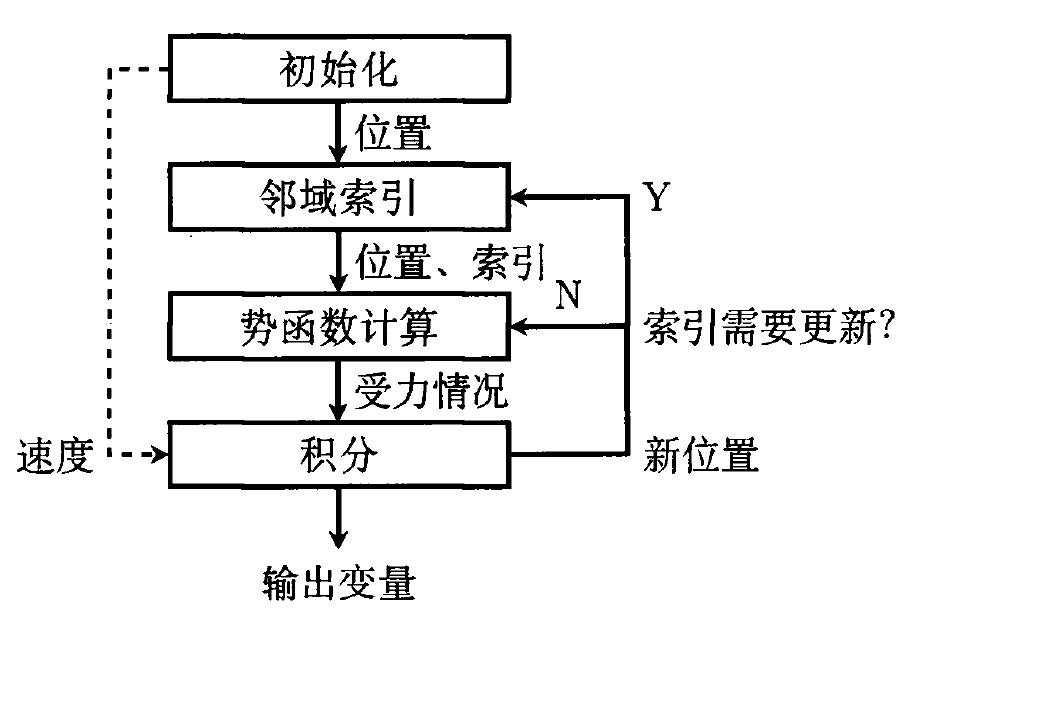
\includegraphics[width=1\textwidth]{2_1.jpg}
  \caption{分子动力学模拟流程图}
\end{figure}

 电子力场势函数与传统方法最大的不同,就是加入了对电子的计算,此时势函数也有了较大的变化,如公式(2-4)所示,在计算原子的物理参数的基础上,还需要对波包及其中的电子进行分析:

 \begin{equation}
   V(R,r,s)=E_{ee}(r,s)+E_{NN}(R)+E_{Ne}(R,r,s)
\end{equation}

其中 𝐸𝑒𝑒 代表不同电子之间的作用力,𝐸𝑁𝑒 代表原子核和电子之间的作用力,𝐸𝑁𝑁 为原子核之间的作用力。

对于经典分子动力学来讲,电子自身以点电荷的形态表示,其在空间内不计算体积,这样就会导致多个电子在趋近于同一位置时,产生位置的重叠导致受力计算不正确,从而产生结果的错误。但在电子力场势函数方法中,由于引入了波包的计算,导致相邻的电子受力始终是一个有限的值,而不会使最终的结果发散。


\subsection{电子力场势函数控制方程解法}
\paragraph{控制方程的解法}
对于计算粒子运动位置和轨迹信息,常用的数值积分方法有 Verlet 算法, Leapfrog 算法[25] 和 Gear Predictor-Corrector 算法[26],其中 Verlet 算法计算速度快,性能好,并且可以占用较少的存储空间。但是计算不够精确,有较大的误差,在进行大规模计算时可能会出现问题。下面是 Verlet 的算法公式:

\begin{equation}
  r(t+\triangle t)=2r(t)-r(t-\triangle t)+\triangle t^2a(t)
  \end{equation}

Leapfrog 算法能够准确算出结果信息,但由于其在计算中无法对速度与位置进行同步,所以无法反应整个体系中同一时刻的距离与粒子轨迹。Gear Predictor-Correct 算法是一种高维算法,其结果准确性高,误差小,但是比较费时,也同时会占用大量的存储空间。

\paragraph{时间步长的确定}
在进行电子力场势函数的计算之前,应当确定合适的时间步长进行模拟。这样能够保证计算精度,又可以获得优秀的计算性能,但对于不同粒子的计算,时间步长的选取是不尽相同的,所以这里选择通过测试用例的实时选取合适的时间步长。

 \begin{figure}[h]
  \centering
  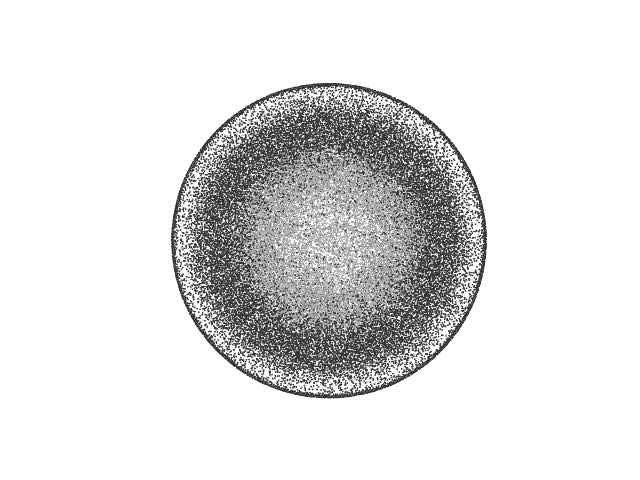
\includegraphics[width=1\textwidth]{2_2.jpg}
  \caption{LAMMPS 中 Li-H2 碰撞模拟过程}
\end{figure}

\section{LAMMPS 计算平台介绍}
\subsection{LAMMPS 软件介绍}
LAMMPS(Large-scale Atomic/Molecular Massively Parallel Simulator)作为分子动力学计算领域内模拟体系涵盖最广的计算平台之一,由隶属于美国能源部的桑迪亚国家实验室进行开发和维护,可以进行多种体系的分子动力学模拟计算,包括生物大分子的结构微观模拟,合金等复合材料的热稳定性等机械性能。在材料力学中统计温度变化下势能,弹性常数的变化情况,并且提供了涉及多重体系的大量势函数,可以同时模拟出于固液气不同状态下的粒子行为,相比于其他分子动力学软件,例如GROMACS[27],NAMD[28],AMBER[29],CHARMM[30],拥有计算模型丰富,运行性能强大,上手容易等特点,软件代码迭代周期短,主要由 C++ 进行编写,其计算性能出色,已经在许多大型计算机上完成了不同体系下的多类大规模计算。针对并行计算的情况LAMMPS 采用了空间分解的方法将模拟体系划分为多个区域,并将子区域按需分配给不同的处理器进行计算。

LAMMPS 项目在20 世纪90 年代中期开始,直到2004 年给出了第一个开源版本,并且知道如今仍然以相当快的速度进行更新。截至 2021 年 4 月,最新的版本是8APR2021。LAMMPS 在提供大量势函数以及计算力场的基础上,同时也支持大量的硬件加速平台,并且针对这些平台额外编写了众多加速包进行支持,例如Nvidia GPU[31],AMD ROCm[32],Intel CPU 以及Xeon phi[33]。在加速模块中也提供了许多并行方法可供参考,如CUDA,OpenCL,ROCm HIP,OpenMP, MPI 等。LAMMPS 本身也对通用 CPU 的多种向量化指令集提供了支持,包括SSE2[34],AVX256[35],AVX512[36] 等。

\subsection{LAMMPS 工作流程介绍}
LAMMPS 的主要工作流程大致可分为三部分:初始化过程,模拟与计算,数据的后处理过程。

\subsubsection{初始化过程}
首先生成输入数据文件,这里可以根据计算模拟的体系与类型来控制数据文件,可以使用 matlab 进行数据文件的生成,其中包括体系中粒子的规模,类型个数,所分布区域的范围,然后为每个粒子设置相关参数,包括初始化位置坐标,自旋类型,编号及带电量等。接下来再编写输入配置文件,可以在配置文件中通过编写计算参数来模拟不同的计算过程,主要包括设置边界条件,时间步长,续算文件的控制,还可以描述输出结果的频率与所在模拟过程的系综。

\subsubsection{模拟与计算过程}
通过输入文件将体系中的粒子数据读入并形成完整的初始体系,首先利用Minimize 过程进行能量最小化的步骤,使其达到一个能够模拟稳定的初始状态,然后通过设置温度来为体系中所有粒子赋一个初速度,粒子开始无规则运动并进行一定时间步的弛豫过程,使粒子出于一个分散的状态,之后通过对体系边界的收缩产生激波使粒子随激波进行定向运动。在整个模拟过程中以牛顿定律为基础,通过对粒子间作用力的变化产生加速度与速度的改变,最后再把每个周期粒子信息记录下来,形成完整的运动轨迹。通过电子力场势函数完成对粒子间作用力的计算是最复杂也最耗时的部分,而在并行计算的过程中,通信的时间也占用了不小的比例。在完成每个时间步作用力的计算后,由于粒子的坐标位置不断变化,粒子对应的邻接表信息也会发生改变。过大的时间步长会使模拟的计算结果发散,所以这里选择△t = 0.005fs 作为整体计算的时间步长,而完成整个模拟计算则至少需要几十万的时间步。

\subsubsection{后处理过程}
在完成各个阶段的计算之后,LAMMPS 会给出多个不同类型的输出文件来对整个模拟过程进行量化的描述,以供后续的处理和分析。其中包括结果日志文件,结构文件,不同粒子的轨迹文件,续算文件等。再通过可视化工具对计算结果进行基本的分析处理,并验证结果的正确性。可视化工具包括OVITO,VMD等。这里能够获得在不同的模拟阶段不同类型粒子结构的运动轨迹和状态,最后通过 matlab 或 python 脚本完成粒子的多角度统计和分析。

 \begin{figure}[h]
  \centering
  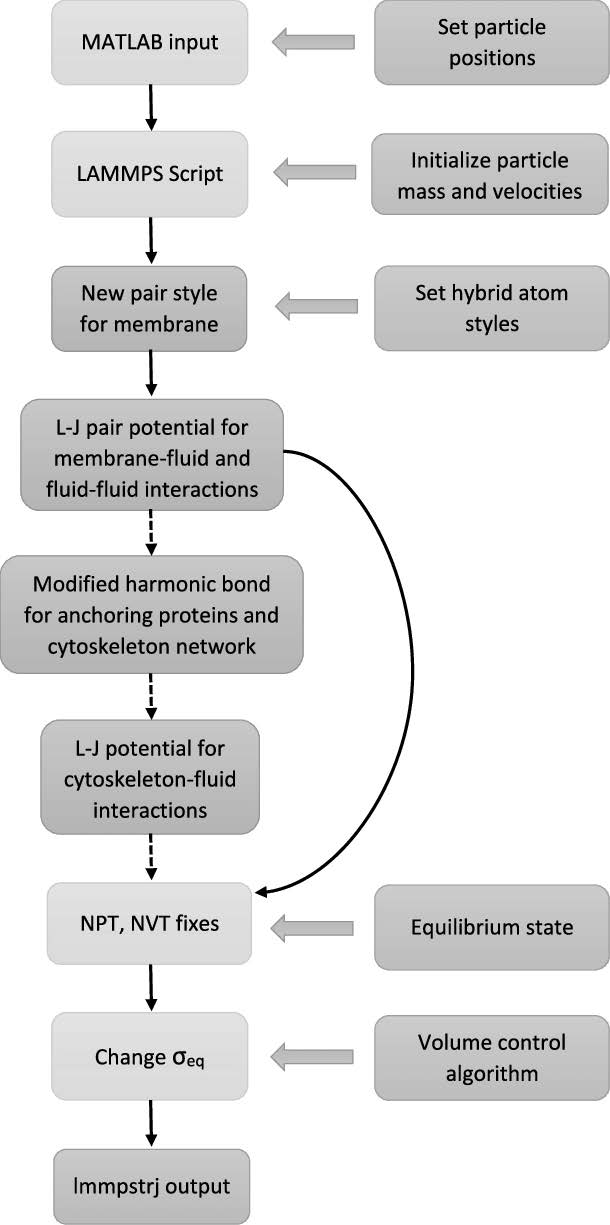
\includegraphics[width=0.5\textwidth]{2_3.jpg}
  \caption{LAMMPS 模拟流程图}
\end{figure}

\section{LAMMPS 在不同平台上的并行实现}
\subsection{LAMMPS 在同构多核处理器上的并行实现}
对于LAMMPS 计算的大规模并行,传统并行计算是在通用同构多核处理器上首先实现的,包括 Intel CPU 以及 Xeon phi 等。并且也累积了不同优化算法和加速包进行支持,其中有 USER-INTEL,USER-OMP 等包。在进行大规模粒子体系的计算时,LAMMPS 首先会对整个体系进行划分,成为域分解(Domain Decomposition), 再将分解后的不同区域放到对应的计算进程上执行。此时该进程只负责对所划分的粒子进行受力计算,并当在所有进程完成计算之后,进行进程间通信并统计粒子受力,体系的压强和温度等关键信息,在进行粒子位置坐标的更新。每当完成固定的时间步计算之后,可以通过负载均衡方法根据粒子密度均匀划分粒子所在的计算区域,使每个进程在每个时间步的耗时相近,这种负载均衡甚至能够得到超过百分之 50 的性能提升。通过处理器硬件支持的同时多线程计算(Simultaneous multithreading,SMT),可以在其中一个线程因为访存等原因处于阻塞时,调用另外一个线程继续执行来保证流水线的高效运行。

与通用多核处理器类似,申威众核处理器也可以通过不同的并行方法实现大规模计算的不同方案并行。例如通过OpenMP 进行单个处理器内的并行,利用MPI 进行大规模节点间的并行。对于科学应用的简单移植,可以只利用SW26010处理器上的单个核组内的主核进行任务的计算和调度工作,期间从核并不参与整个计算,再结合不同并行方法完成整个过程。这种方法类似于在通用处理器环境下的并行实现,但由于 SW26010 处理器主核的设计相对于通用处理器核心计算能力不同强大,其核心频率较低,Cache 容量和层次也相对不足,流水线设计也相对有限,所以这种模式的计算性能往往相对较弱,但对于 SW26010 处理器的设计理念来讲,充分利用从核阵列才是提升计算性能的关键,所以在软件移植的基础上,还要将热点计算集成到从核阵列上,并充分利用 SW26010 处理器的硬件特性与优化措施,针对 LAMMPS 计算进行特定的并行方案设计。

 \begin{figure}[h]
  \centering
  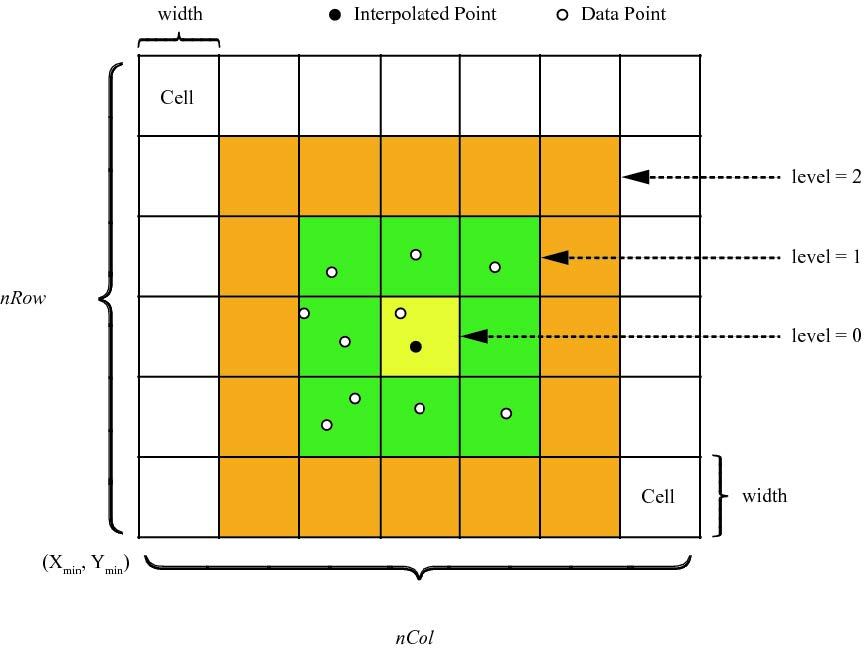
\includegraphics[width=0.5\textwidth]{2_4.jpg}
  \caption{LAMMPS 采用空间分解分配模拟区域}
\end{figure}

\subsection{LAMMPS 在异构 CPU-GPU 平台上的并行实现}
GPU(Graphics processing unit)最初是作为图形处理硬件来进行图形图象的像素处理,其上的 GPU 处理阵列和帧缓冲存储接口也是为处理图形数据而设计的,但随着大量的浮点和整数处理器的加入,结构也转向了通用的并行变成体系结构。对比于CPU 复杂的片上结构和指令集设计,GPU 凭借大量的计算单元的集成和更高的存储带宽设计占据了大量通用计算的领域市场,当前学术和工业领域的多类计算已经开始转向 GPU 平台,包括并不限于分子动力学模拟,金融计算等。并且 GPU 对不同精度的计算需要也都能够满足。对于分子动力学计算的大规模并行,LAMMPS 也提供了不同的优化算法和加速包进行支持,包括GPU 和 KOKKOS 加速包。在进行计算时,LAMMPS 会将势函数受力的计算加载到GPU 上去执行,并在多时间步的迭代中,完成在GPU 端进行计算,此时计算粒子的信息,包括受力,类型,位置坐标,并不需要在CPU 和GPU 上来回传递,这样做保证了通信性能的同时也提高了计算效率,这种方法在计算大规模体系时性能优势更加明显,并且在GPU 进行势函数计算时,CPU 不需要进行等待,仍可以进行 I/O 操作,通信等方面的处理工作。邻接表同时也可在 GPU 端直接进行构造,无需 CPU 的参与。在使用 Nvidia Tesla GPU 对计算进行并行计算时,性能可比Xeon E5 处理器快三倍以上。SW26010 处理器与GPU 的结构和计算分布类似,都是将核心势函数计算加载到多核器件上运行,但由于申威处理器从核阵列与 GPU 在指令集与硬件架构上有着明显的差异,所以说对于从核线程级并行设计需要提供一套与 GPU 完全不同的并行计算方案。

\section{本章小结}
本章主要介绍了分子动力学计算的基础方法,电子力场势函数eFF 的基本推导以及分子动力学平台LAMMPS 在不同架构计算平台上的并行实现方案。首先,第一节给出了分子动力学计算的物理模型,在经典动力学计算方法中延伸出来的电子立场势函数的分析方法和相关控制方程的解法。第二节介绍了LAMMPS 平台的发展过程,特点以及相关工作流程,简单认识了分子动力学软件 LAMMPS的基本计算策略。第三节讨论了分子动力学软件LAMMPS 在通用多核处理器上的并行方案,以及在异构多核GPU 上的计算方法。相比于通用同构的CPU 处理器,在申威处理器上的优化重点则是利用从核加速阵列,进行细粒度的任务划分和计算分配,而与 GPU 的优化方式不同,申威平台上的计算通过有限的存储空间,高效的计算单元,并结合硬件架构设计合理的通信控制和计算优化方案。
